
Projektis kasutatud spordikell on Polar RC3 GPS.
Konkreetne mudel on toodetud aastal 2013.
Kella tähtsaim omadus on integreeritud GPS moodul, mis suudab arvet pidada tegevuse alguspunkti üle ning kasutajat sinna tagasi suunata, täpsemalt kiirust ja distantsi mõõta.
Lisaks on kell ühilduv mitmete lisasensoritega, millega saab mõõta südametööd, rattasõidu andmeid ja seega koguda veel rohkem treeningu kohta andmeid, millega enda arengut jälgida.
Tehnilistest omadustest on kõige märkimisväärsem kella täpsus +/- 0,5 sekundit päevas ning GPS mooduli täpsus +/-2\% vahemaale ja +/-2km/h kiirusele.\cite{rc3-man}

\begin{figure}[ht]
    \centering
    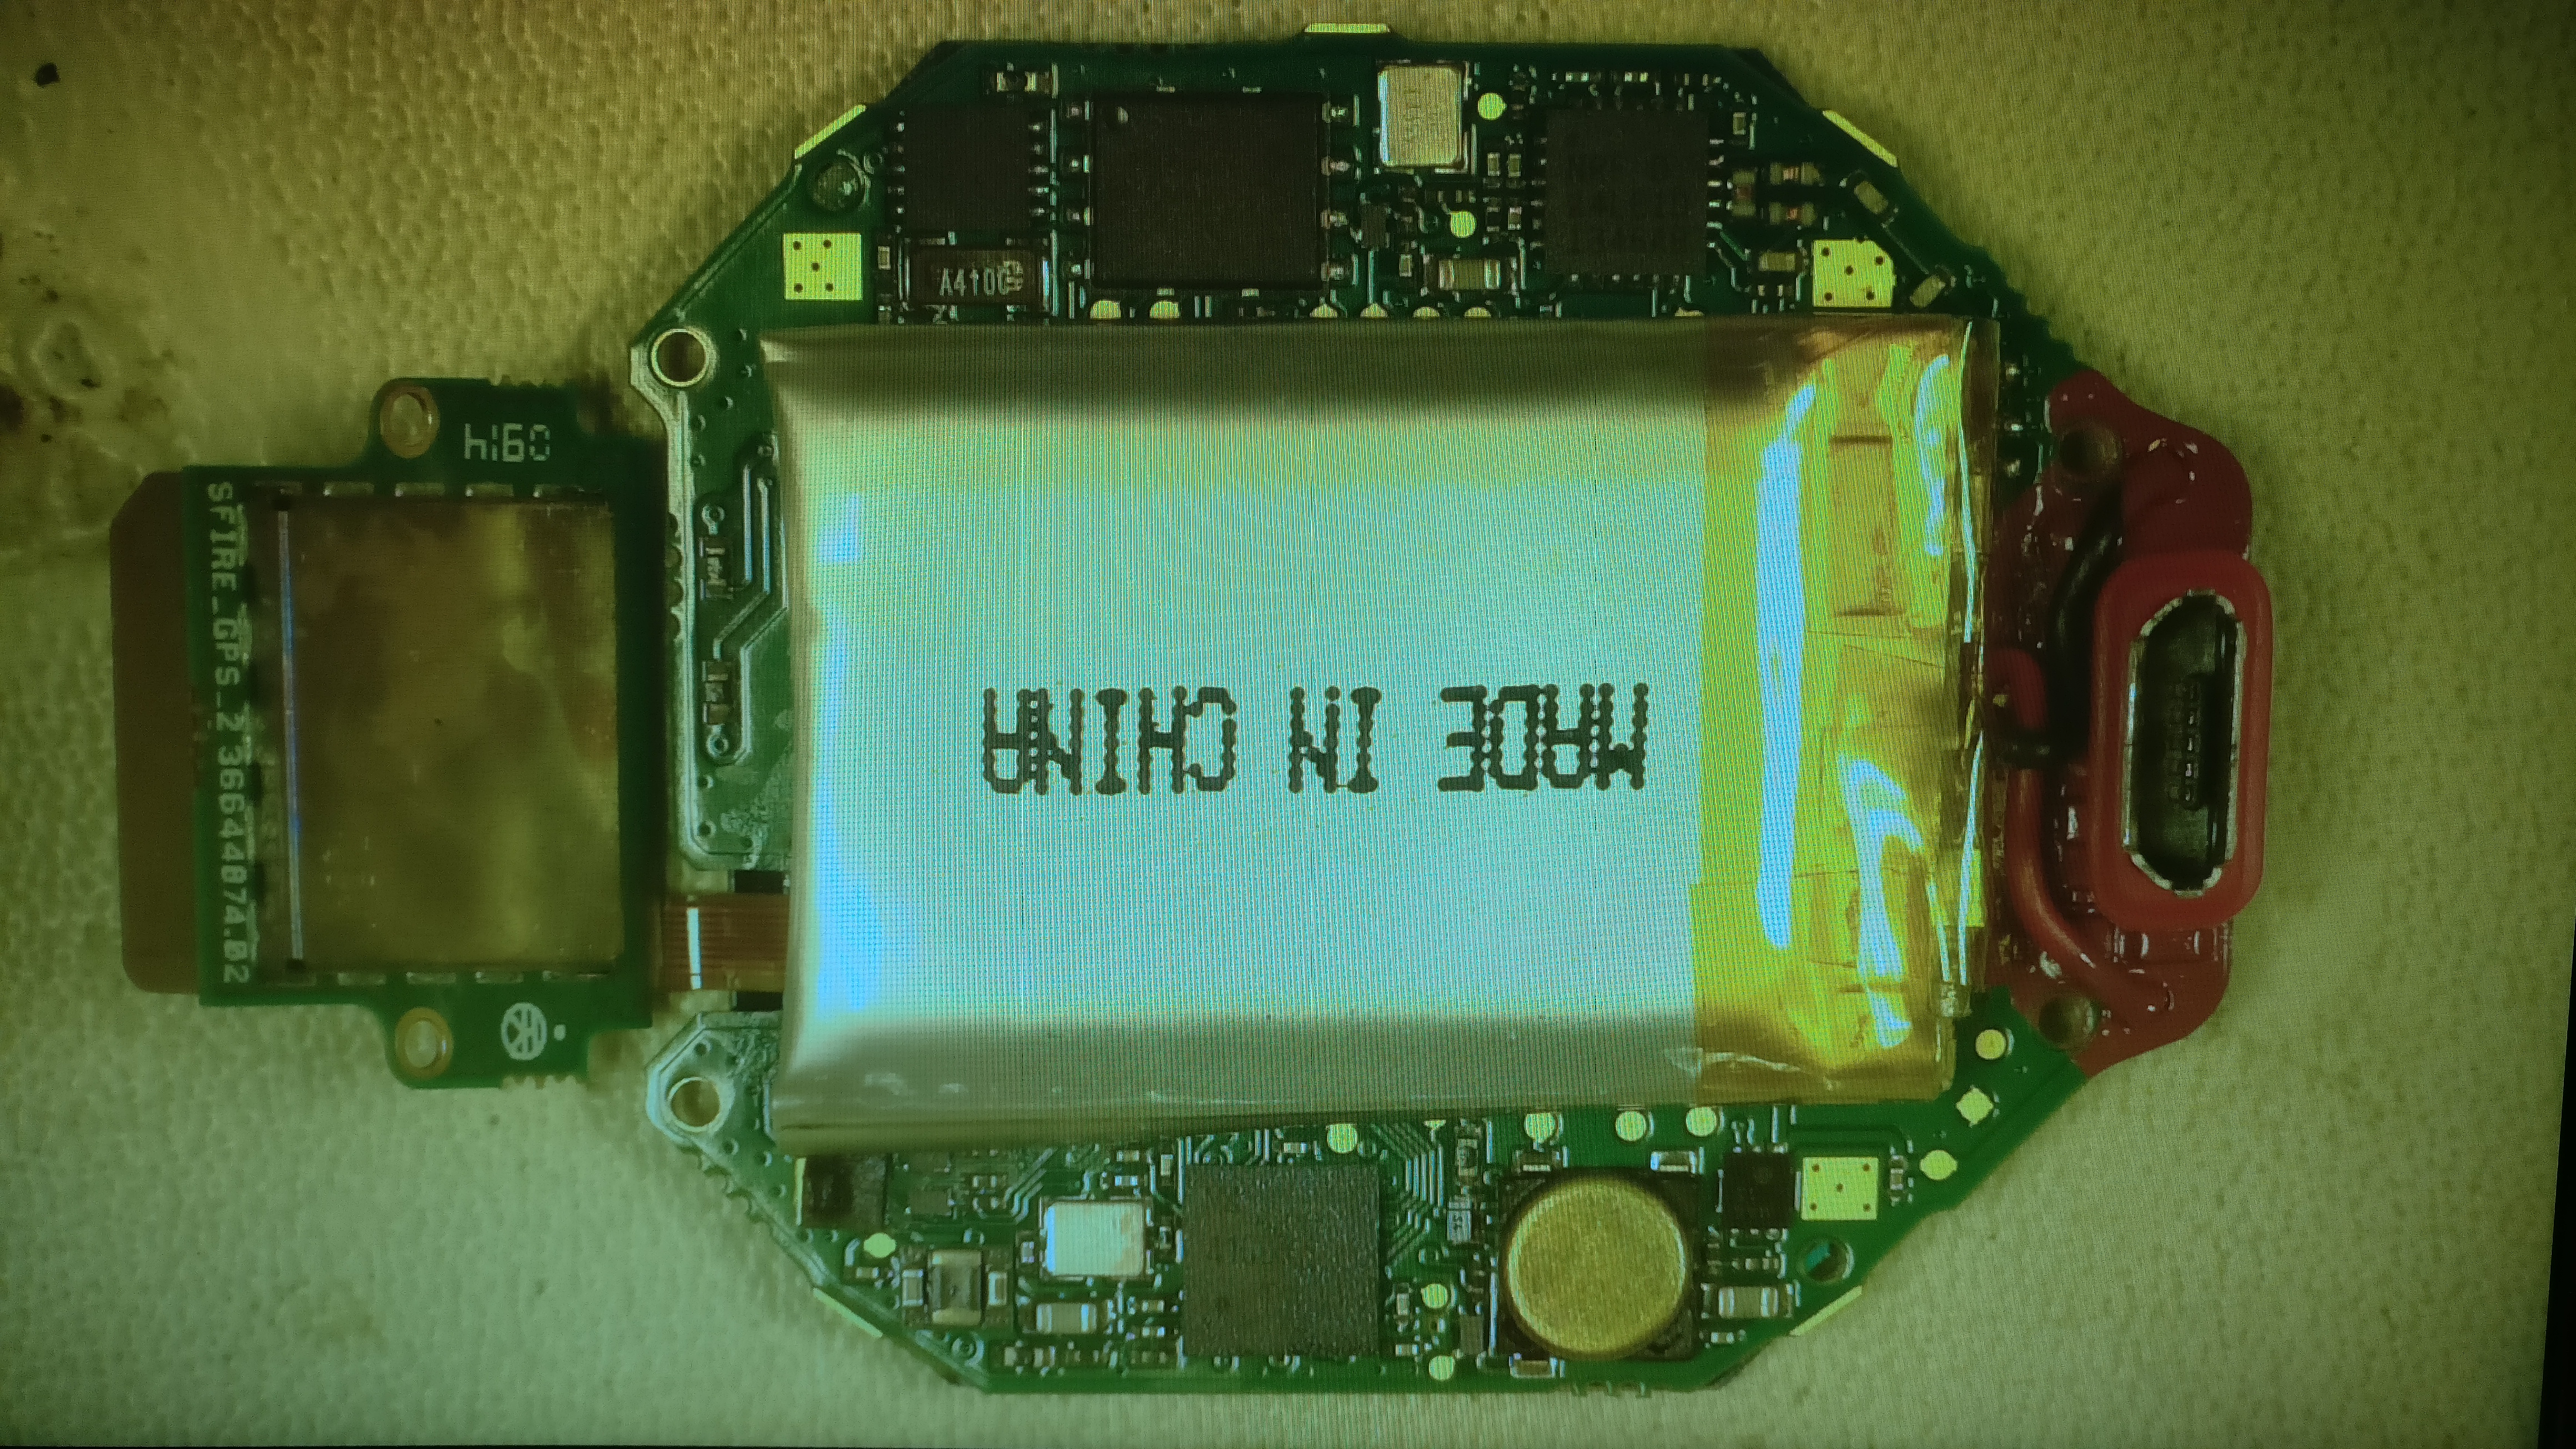
\includegraphics[width=.7\textwidth]{figures/watch.jpg}
    \caption{\textit{Pilt kella sisemusest}}
    \label{fig:watch}
\end{figure}

Projekti alguses tutvuti ka kella riistvaraga, võttes kell lahti ja uurides selle komponente ning otsides andmeliine, mida oleks lihtne füüsiliselt jälgida, et saada paremini aru kella töötamisest.
Kella pidi saama ka hiljem kasutada, mistõttu ei hakatud antud projekti käigus eemaldama kella komponente emaplaadilt, et neid lähemalt uurida.

Kella riistvara kohta dokumentatsiooni ei leitud ning kella enda emaplaati uurides ka ei olnud lihtne aru saada, millised konkreetsed komponendid sellel kasutatud olid ja mis eesmärk igal detailil oli.
Kella uuriti mikroskoobi all ning iga komponendi kohta pandi kirja kogu informatsioon, mis oli võimalik leida visuaalsel vaatlusel.

\begin{figure}[ht]
    \centering
    \includegraphics[width=.5\textwidth]{figures/kella-komponendid.jpg}
    \caption{\textit{Skeem komponentidest nende peale loetud informatsiooniga}}
    \label{fig:components}
\end{figure}

Joonisel~\ref{fig:components} on kujutatud kella pealt leitud komponendid nende peal olnud informatsiooniga samas asetuses nagu ka Joonisel~\ref{fig:watch}.
Komponente uurides eeldati, et komponendid 1 ja 6 on kellad, kuna nende peal olev tekst viitab sagedusele ning on ka levinud kasutada konkreetseid eraldiseidvaid kellasid mikroskeemides, kus ajaline täpsus on oluline.
Komponent numbriga 3 oli ainus komponent, mille peal polnud midagi kirjas.
Komponentidest 2, 5 või 7 on üks ilmselt põhiline protsessor, kuigi ei õnnestunud kindlaks teha milline see neist täpselt olla võiks.
